\section{Planung und Vorbereitung}
Für die Planung eines Videos benötigt man meistens viel Zeit, um auch ein gutes Ergebnis zu erzielen. Bevor es an das bekannte Drehbuch geht, muss man vorerst noch drei andere Schritte berücksichtigen, nämlich die sogenannte Logline, das Expos\'{e} und das Treatment. Erst nach diesen Schritten ist es sinnvoll das Drehbuch zu schreiben.\citep{planung}
\subsection{Logline}
Die Logline ist, vereinfacht gesagt, die Idee zum Film oder zum Video. Die Logline besteht meistens nur aus einem Satz und soll nur einen groben Überblick über den Film oder des Videos preisgeben.\citep{logline}
\begin{figure}[H]
	\centering
	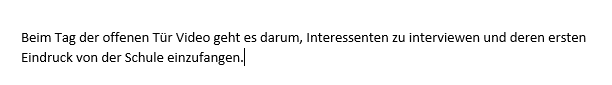
\includegraphics[width=1.0\textwidth]{abb26} 
	\caption{Logline des Tag der offenen Tür Videos}
\end{figure}
\subsection{Expos\'{e}}
Das Expos\'{e} besteht meist nur aus ein paar Skizzen, wobei folgende Themen behandelt werden: das Thema selbst, die Besonderheiten des Videos oder Films, die Protagonisten, Drehorte und sonstige Herausforderungen. Das Expos\'{e} soll den Mitarbeitern dazu dienen, weitere Entscheidungen leichter zu treffen.\citep{expose}
\subsection{Treatment}
Das Treatment ist mehr oder weniger der Vorgänger des Drehbuchs. Ein Treatment beinhaltet schon kurze Dialoge zu bestimmten Szenen und eine szenengenaue Auflösung zum Film oder zum Video.\citep{treatment}
\subsection{Drehbuch}
Das Drehbuch ist, im Vergleich zum Treatment, komplett ausgearbeitet, das heißt, es liegt ein kompletter Produktionsleitfaden vor, wobei jede Szene ausgearbeitet ist. Weiters werden wichtige Einstellungen in Bildszenen dargestellt. Adobe bietet die kostenlose Software \textit{Story} an, mit der man Drehbücher erstellen kann.\citep{drehbuch}\newline
Story ist eine Software von Abdobe, mit der man Drehbücher erstellen kann. Bei der Erstellung kann man ein vorgefertigtes Template auswählen und anschließend kann man schon das Drehbuch verfassen. Bei der Erstellung des Drehbuchs kann man zwischen Scene Heading, Action, Character, Parenthetical, Dialog, Transition, Speaking Extra, Shot und General auswählen. Diese Elementtypen sind auch schon dementsprechend formatiert und man muss weder etwas einrücken, noch sonstige Formatierungen einstellen.\citep{drehbuchZwei}\\ 
Da nur Interviews geplant wurden und man bei Interviews keine Szenen planen kann, wurde das Expos\'{e}, das Treatment und das Drehbuch übersprungen. Jedoch wurde eine Logline und das Storyboard verfasst und zusätzlich wurde noch ein Fragenkatalog pro Video erstellt. 
\subsection{Storyboard}
Ein Storyboard ist eine visualisierte Veranschaulichung von dem Konzept, das man sich zuvor überlegt hat.\citep{storyboard} Um die korrekte Ausführung der Videos zu gewährleisten, wurden Storyboards angefertigt. Diese wurden mit der Online Plattform "Storyboard That"\citep{storyboardLink} erstellt und schließlich als PDF - Format exportiert.
Im Storyboard wurden die Szenen bildlich dargestellt, was das Team im weiteren Verlauf unterstützte, da es dadurch grobe Fehler vermeiden konnte.
Das Online - Tool ermöglichte es zwischen verschiedensten Szenen, Charakteren und Kategorien auszuwählen, wodurch vereinfacht, verschiedenste Szenen dargestellt werden konnten. 
\begin{figure}[H]
\begin{center}
	\fbox{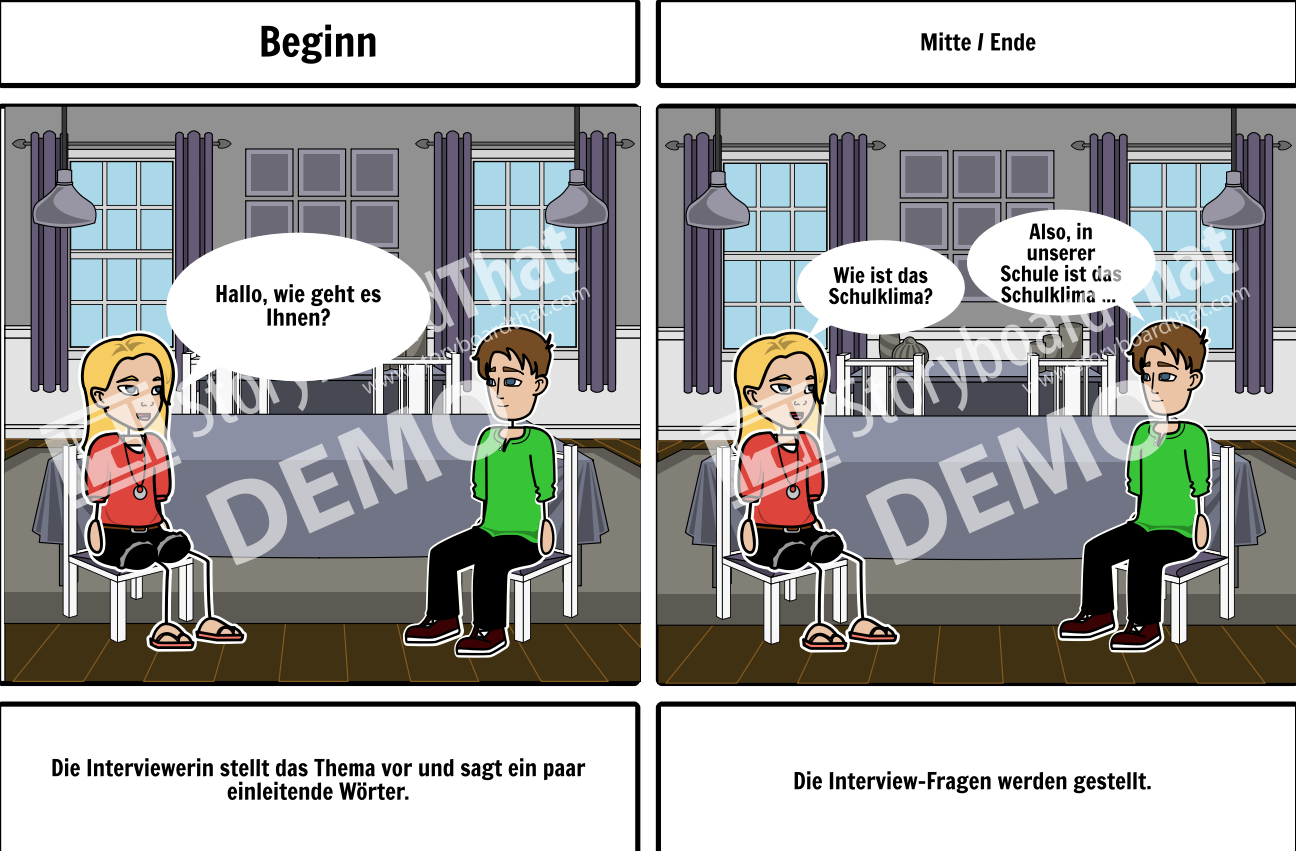
\includegraphics[scale=0.30]{abb10}}
	\caption{Storyboard des Interviews mit dem Abteilungsvorstand}
\end{center}
\end{figure}